%%%%%%%%%%%%%%%%%%%%%%%%%%%%%%%%%%%%%%%%%%%%%%%%%%%%%%%%%%%%%%%%%%%%%%%%%%%%%%%%%%%%%%%%%%%%%%%%%%%%%%%%%%
%Write by:ShuwenHe
%Date:20230613
%%%%%%%%%%%%%%%%%%%%%%%%%%%%%%%%%%%%%%%%%%%%%%%%%%%%%%%%%%%%%%%%%%%%%%%%%%%%%%%%%%%%%%%%%%%%%%%%%%%%%%%%%%

%%%%%%%%%%%%%%%%%%%%%%%%%%%%%%%%%%%%%%%%%%%%%%%%%%%%%%%%%%%%%%%%%%%%%%%%%%%%%%%%%%%%%%%%%%%%%%%%%%%%%%%%%%
\documentclass[12pt,twiside,a4paper]{ctexbook}
\usepackage[centertags]{amsmath}
\usepackage{amsfonts}
\usepackage{amsthm}
\usepackage{newlfont}
\usepackage{makeidx}
\usepackage{wasysym}
\usepackage{geometry} 
\usepackage{graphics}
\usepackage{ulem}
\usepackage{slashbox} 
\usepackage{fancyhdr} 
\usepackage[pdftex]{graphicx}
\usepackage{epstopdf}
\usepackage{cite}
\usepackage{listings}
\usepackage{tocbibind}
\usepackage[numbers,sort&compress]{natbib}

\setlength\parskip{\baselineskip}
\setcounter{tocdepth}{8} % 生成目录层级
\setcounter{secnumdepth}{4}
\renewcommand\thesection{\arabic{section}}
\usepackage[pdfstartview=FitH,CJKbookmarks=true,bookmarks,bookmarksnumbered=true,
    colorlinks=true,citecolor=black,linkcolor=black,anchorcolor=green,urlcolor=black]{hyperref}
\usepackage{titlesec}
\titleformat{\chapter}[display]{\normalfont\huge\bfseries\center}{\chaptertitlename}{1pt}{\Huge}
\titleformat{\section}{\normalfont\Large\bfseries}{\thesection}{1em}{}
\titleformat{\subsection}{\normalfont\large\bfseries}{\thesubsection}{1em}{}
\titleformat{\subsubsection}{\normalfont\normalsize\bfseries}{\thesubsubsection}{1em}{}
\titleformat{\paragraph}[runin]{\normalfont\normalsize\bfseries}{\theparagraph}{1em}{}
\titleformat{\subparagraph}[runin]{\normalfont\normalsize\bfseries}{\thesubparagraph}{1em}{}
\titlespacing*{\chapter} {0pt}{10pt}{10pt}
\titlespacing*{\section} {0pt}{0.5ex plus 1ex minus .2ex}{0.3ex plus .2ex}
\titlespacing*{\subsection} {0pt}{0.25ex plus 1ex minus .1ex}{0.5ex plus .1ex}
\titlespacing*{\subsubsection}{0pt}{3.25ex plus 1ex minus .2ex}{1.5ex plus .2ex}
\titlespacing*{\paragraph} {0pt}{3.25ex plus 1ex minus .2ex}{1em}
\titlespacing*{\subparagraph} {\parindent}{3.25ex plus 1ex minus .2ex}{1em}
\numberwithin{chapter}{part}
\geometry{left=2.0cm,right=20mm,top=25mm,bottom=25mm}
\let\cleardoublepage\clearpage
%%%%%%%%%%%%%%%%%%%%%%%%%%%%%%%%%%%%%%%%%%%%%%%%%%%%%%%%%%%%%%%%%%%%%%%%%%%%%%%%%%%%%%%%%%%%%%%%%%%%%%%%%%

%%%%%%%%%%%%%%%%%%%%%%%%%%%%%%%%%%%%%%%%%%%%%%%%%%%%%%%%%%%%%%%%%%%%%%%%%%%%%%%%%%%%%%%%%%%%%%%%%%%%%%%%%%
%mathematics
\usepackage{amssymb}
\usepackage{diagbox}
%%%%%%%%%%%%%%%%%%%%%%%%%%%%%%%%%%%%%%%%%%%%%%%%%%%%%%%%%%%%%%%%%%%%%%%%%%%%%%%%%%%%%%%%%%%%%%%%%%%%%%%%%%

%%%%%%%%%%%%%%%%%%%%%%%%%%%%%%%%%%%%%%%%%%%%%%%%%%%%%%%%%%%%%%%%%%%%%%%%%%%%%%%%%%%%%%%%%%%%%%%%%%%%%%%%%%
%
%%%%%%%%%%%%%%%%%%%%%%%%%%%%%%%%%%%%%%%%%%%%%%%%%%%%%%%%%%%%%%%%%%%%%%%%%%%%%%%%%%%%%%%%%%%%%%%%%%%%%%%%%%

%%%%%%%%%%%%%%%%%%%%%%%%%%%%%%%%%%%%%%%%%%%%%%%%%%%%%%%%%%%%%%%%%%%%%%%%%%%%%%%%%%%%%%%%%%%%%%%%%%%%%%%%%%
%
\usepackage{tipa}
%%%%%%%%%%%%%%%%%%%%%%%%%%%%%%%%%%%%%%%%%%%%%%%%%%%%%%%%%%%%%%%%%%%%%%%%%%%%%%%%%%%%%%%%%%%%%%%%%%%%%%%%%%

%%%%%%%%%%%%%%%%%%%%%%%%%%%%%%%%%%%%%%%%%%%%%%%%%%%%%%%%%%%%%%%%%%%%%%%%%%%%%%%%%%%%%%%%%%%%%%%%%%%%%%%%%%
\begin{document}
%%%%%%%%%%%%%%%%%%%%%%%%%%%%%%%%%%%%%%%%%%%%%%%%%%%%%%%%%%%%%%%%%%%%%%%%%%%%%%%%%%%%%%%%%%%%%%%%%%%%%%%%%%

%\author
%{
%Peking University\\
%北京大学\\
%ShuwenHe\\
%何书文\\
%1201220707@pku.edu.cn
%}

%%%%%%%%%%%%%%%%%%%%%%%%%%%%%%%%%%%%%%%%%%%%%%%%%%%%%%%%%%%%%%%%%%%%%%%%%%%%%%%%%%%%%%%%%%%%%%%%%%%%%%%%%%
%\centerline{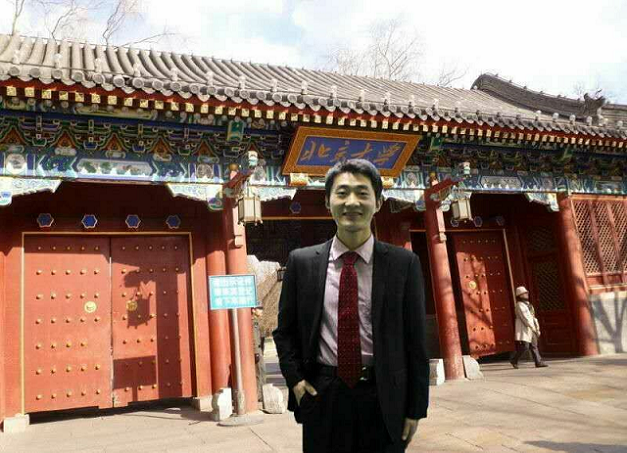
\includegraphics{shuwenhe.png}}
%写好一本书:工匠精神!用心打造!夜深写于北京大学图书馆。作者亲自一线带课,所带学生多人保送或考入清华北大,根据多年清华附中、101中学、人大附中、北大附中、十一学校,考试真题分析经验所得。用此书考上心目中名校学生无数!何书文北京大学硕士,资深数学名师、信息学竞赛算法名师,所带学生多名考入人大附中早培、清华附中优才、101 实验班、北大附中实验班等名校。全国中学数学联赛、全国中学数学竞赛的辅导老师,全国NOI、CSP信息学竞赛辅导名师。何书文老师在北京大学学习期间立志从事教育事业,帮学生授业解惑。何书文老师小学期间学习奥数,并多次获奖,为以后的学习与研究打下良好基础。何书文 老师在中学阶段数学、物理均获奖。何书文老师在小学中学期间一直为数学课代表,中小学大学期间担任班长,何书文老师在北京大学被选为科技一苑苑长,组织北大同学积极参与校各项活动,积极参与校学生会工作,何书文老师被北京大学评为优秀入党积极分子.何书文老师经常参加北京大学数学课题的研讨班。何书文 老师是北京大学数学系暑期学校全国选出40 名优秀中青年数学人才之一,参加伦敦国王学院、美国杜克大学、美国纽约大学、加拿大多伦多大学教授组成的学术研讨班,研究PDE(偏微分方程),量子力学方面的数学课题的研究工作,并获得优异成绩结业。何书文老师作为项目经理用数学建模方法给大型企业开发软件,用数学方法规划提高企业产能协作效率。何书文 老师致力于数学方面的教学与研究工作,所带多名孩子已经被点优才进入清华附中创新班,101 实验班,人大附中早培班,是家长值得信赖的老师。考上学生继续跟随何书文老师学习全国数学联赛,全国数学竞赛系列课程,同时学习NOI、IOI、ACM算法编程竞赛。
%%%%%%%%%%%%%%%%%%%%%%%%%%%%%%%%%%%%%%%%%%%%%%%%%%%%%%%%%%%%%%%%%%%%%%%%%%%%%%%%%%%%%%%%%%%%%%%%%%%%%%%%%%

%%%%%%%%%%%%%%%%%%%%%%%%%%%%%%%%%%%%%%%%%%%%%%%%%%%%%%%%%%%%%%%%%%%%%%%%%%%%%%%%%%%%%%%%%%%%%%%%%%%%%%%%%%
\title{Quiz}
%\maketitle
%\tableofcontents % 显示目录
%\newpage
\pagestyle{fancy}
%%%%%%%%%%%%%%%%%%%%%%%%%%%%%%%%%%%%%%%%%%%%%%%%%%%%%%%%%%%%%%%%%%%%%%%%%%%%%%%%%%%%%%%%%%%%%%%%%%%%%%%%%%

%\lhead{
\includegraphics{shuwenedu.png}}
%\rhead{改变您家孩子命运的老师}
%\lfoot{
\includegraphics{pku.png}算法第一人北大何书文}
%\rfoot{升学规划 何校长 电话微信15010729356}
%%%%%%%%%%%%%%%%%%%%%%%%%%%%%%%%%%%%%%%%%%%%%%%%%%%%%%%%%%%%%%%%%%%%%%%%%%%%%%%%%%%%%%%%%%%%%%%%%%%%%%%%%%

%%%%%%%%%%%%%%%%%%%%%%%%%%%%%%%%%%%%%%%%%%%%%%%%%%%%%%%%%%%%%%%%%%%%%%%%%%%%%%%%%%%%%%%%%%%%%%%%%%%%%%%%%%
%\chapter{csp-j}
\section{}
小文同学刚刚接触了信息学竞赛,有一天她遇到了这样一个题:给定正整数a和b,求$a^b$的值是多少。\\
$a^b$即b个a相乘的值,例如$2^3$即为3个2相乘,结果为$2\times2\times2=8$。\\
“简单!”小文心想,同时很快就写出了一份程序,可是测试时却出现了错误。\\
小文很快意识到,她的程序里的变量都是 int 类型的。在大多数机器上,int 类型
能表示的最大数为$2^{31}−1$,因此只要计算结果超过这个数,她的程序就会出现错误。\\
由于小文刚刚学会编程,她担心使用 int 计算会出现问题。因此她希望你在 $a^b$ 的
值超过 $10^9$ 时,输出一个 ‐1 进行警示,否则就输出正确的 $a^b$ 的值。\\
然而小文还是不知道怎么实现这份程序,因此她想请你帮忙。\\
【输入格式】\\
从文件 $pow.in$ 中读入数据。\\
输入共一行,两个正整数 a, b 。\\
【输出格式】\\
输出到文件$pow.out$中。\\
输出共一行,如果 $a^b$ 的值不超过 $10^9$ ,则输出 $a^b$ 的值,否则输出 ‐1 。\\
【样例 1 输入】\\
10 9\\
【样例 1 输出】\\
1000000000\\
\vspace{10cm}

\section{}
小$K$同学向小$P$同学发送了一个长度为8的01字符串来玩数字游戏,小$P$同学想要知道字符串中究竟有多少个1。\\
注意:01字符串为每一个字符是0或者1的字符串,如“101”(不含双引号)为一个长度为3的01字符串。\\
【输入格式】\\
输入文件名为number.in\\
输入文件只有一行,一个长度为8的01字符串$s$。\\
【输出格式】\\
输出文件名为number.out\\
输出文件只有一行,包含一个整数,即01字符串中字符1的个数。\\
【输入输出样例1】\\
\begin{tabular}{|c|c|}
\hline
number.in & number.out\\
\hline
00010100 & 2\\
\hline
\end{tabular}\\
\vspace{11cm}

\section{}
给定一个正整数$k$,有$k$次询问,每次给定三个正整数$n_i, e_i, d_i$求两个正整数$p_i
, q_i$,使$n_i = p_i \times q_i, e_i \times d_i = (p_i − 1)(q_i − 1) + 1$。\\
【输入格式】\\
从文件decode.in中读入数据。\\
第一行一个正整数$k$,表示有$k$次询问。\\
接下来$k$行,第$i$行三个正整数 $n_i, d_i, e_i$。\\
【输出格式】\\
输出到文件 decode.out 中。\\
输出$k$行,每行两个正整数$pi,qi$\\表示答案。\\
为使输出统一,你应当保证 $pi \leq qi$。\\
如果无解,请输出 NO。\\
【样例 1 输入】\\
\begin{tabular}{|c|c|c|}
  \hline
  1 & 10 \\
  2 & 770 77 5 \\
  3 & 633 1 211 \\
  4 & 545 1 499 \\
  5 & 683 3 227\\
  6 & 858 3 257\\
  7 & 723 37 13\\
  8 & 572 26 11\\
  9 & 867 17 17\\
  10 & 829 3 263\\
  11 & 528 4 109\\
  \hline
\end{tabular}\\
【样例 1 输出】\\
\begin{tabular}{|c|c|c|}
  \hline
  1 & 2 385 \\
  2 & NO \\
  3 & NO \\
  4 & NO \\
  5 & 11 78\\
  6 & 3 241\\
  7 & 2 286\\
  8 & NO\\
  9 & NO\\
  10 & 6 88\\
  \hline
\end{tabular}\\
\vspace{10cm}

\section{}
判断prime.in中的数是否是素数,如果是输出1到prime.out否则输出0。

\clearpage
\end{document}
